\clearpage
\section{Experimental Research Designs}
\label{sec:experimental-design}

The aim of this research is detecting road defects using multimodal machine learning. As described earlier in section \ref{section:multimodal-ml}, multimodal means that a modal uses multiple data sources. In this case, we are dealing with visual- and accelerometer data. From research is known that there are typically three moments in the pipeline where the modalities can be fused: early-, middle-, or late fusion \cite{Baltrusaitis2017}. However, we can also create a modal on the distinctive modality. For instance, training a classifier solely using visual data. To this aim we compare the performance of a multimodal machine learning with that of a unimodal machine learner.

This means that we are developing three different machine learners: 1) model using visual data, 2) model using accelerometer, 3) model using combination of visual and accelerometer data. We refer to the respective experiment designs as \textit{tracks}. The rest of the section will explain the rest of the research. We first explain how the dataset is constructed. Then we describe the evaluation metrics used to compare the models. Followed by section describing the machine learning model for each respective track.

Experiments in the different tracks are executed on the same machine. The machine has the following specifications: Intel Core i7-7700K CPU, NVIDIA GeForce GTX 1080 GPU, and 32 GiB RAM. The machine runs Debian 11 as operating system. Machine learning configurations, training performance, and results are tracked with an open-source tool called Weights and Biases (wandb) \cite{wandb}.


\begin{figure}[ht]
\begin{center}
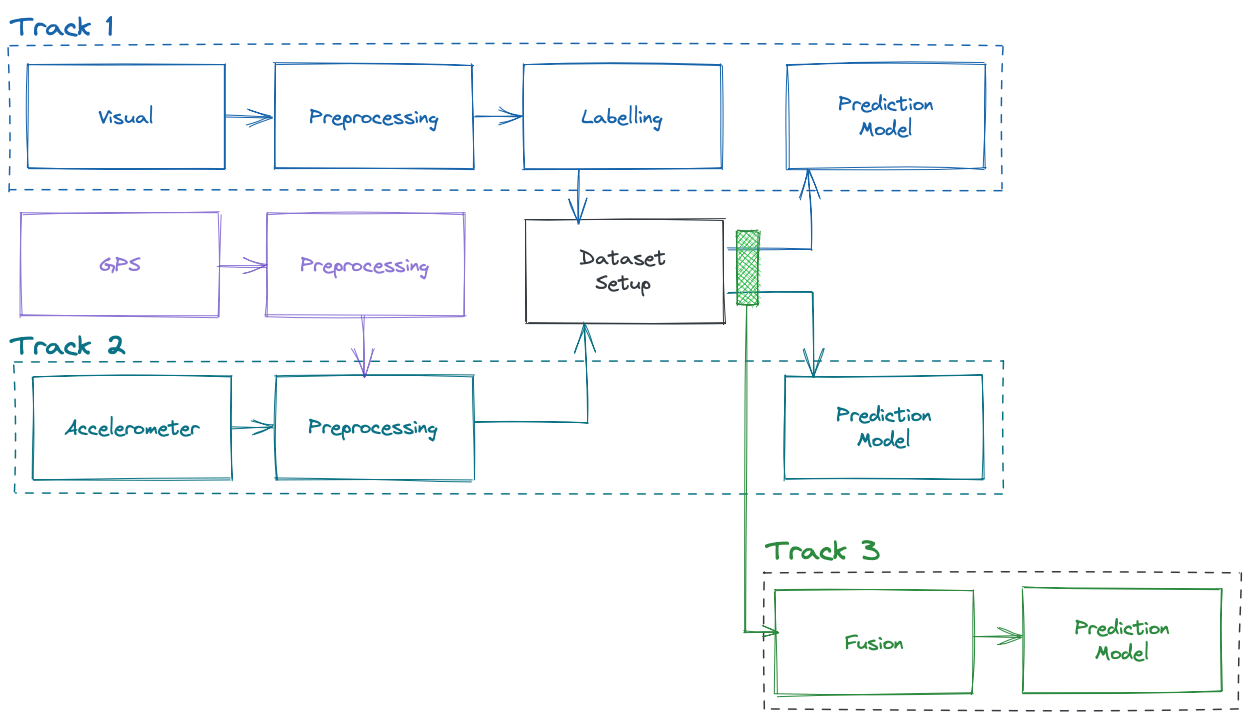
\includegraphics[width=0.95\textwidth,keepaspectratio]{images/5_multimodal_fusion/research-tracks.png}
\captionsetup{width=.95\textwidth}
\caption{Visualization displaying the different research tracks. Each track is a different machine learning model.}
\label{fig:fusion-strategies}
\end{center}
\end{figure}


\subsection{Dataset Setup}
\label{sec:dataset-setup}

In this work we develop three different machine learners using different data types as input. However, to make a comparison between the different machine learners, we create a common dataset that is used in each model. We cannot directly compare the performance of a visual model with that of an accelerometer based model. Both models need to be grounded to the same event. That is, we need to give both models input that covers the same road anomaly to make a valid comparison.

As mentioned earlier, to scope our research, we only look at manholes present on asphalt roads. Asphalt roads cause the least amount of vibrations while driving. It is assumed when noisy data is provided, the accelerometer is unable to learn from the data. Replicating the research on different road types is an interesting direction for future research.

Both data sources are annotated with timestamp of recording. We use this common denominator to segment the data in windows covering a fixed time period. Subsequently we label each segment positively if they contain a manhole, and negatively otherwise. Labelling of the segments uses a heuristic based on the frames of the visual data. 

The target variable of the machine learners is whether a manhole is present in a segment. This makes the task a binary classification problem. The predictive variables depends on the respective research track. For track 1 (visual model) it is the frame. For track 2 (accelerometer model) it is the acceleration signal. And, for track 3 (fusion) it is both the frame and acceleration signal. 

The data is segmented in sliding windows of one second in length, and each segment has an overlap of 50\%. This is shown in figure \ref{fig:segmentation}. Detecting if a manhole is present in a segment is done with the following heuristic. First, we query all frames around the start time of the accelerometer segment. Specifically, we query the frames between $-0.5$ and $+0.2$ seconds. Remember that the visual data detects manholes earlier due the front faced perspective. Secondly, we filter the frames on following criteria: 1) there are one or multiple frames with a manhole, 2) the manhole in the image is detected at location it is likely the wheel drives over, 3) a threshold is used to judge if the segment contains a significant vibration. See listing \ref{list:label_segments} for a pseudo implementation. The window length of one second, and period of selecting the frames was empirically shown effective.

\begin{figure}[ht]
\begin{center}
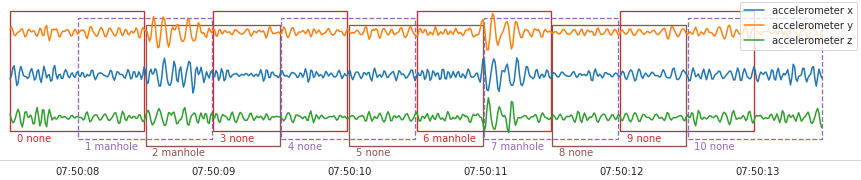
\includegraphics[width=0.95\textwidth,keepaspectratio]{images/5_multimodal_fusion/segment-example.png}
\captionsetup{width=.95\textwidth}
\caption{Example of segmentation. Each window is 100 samples / 1 second in length, and has overlap of 50\%. Note, windows 1 / 2 and 6 / 7 are labelled as manhole. (Coloring of the segments are solely for illustrative purposes.)}
\label{fig:segmentation}
\end{center}
\end{figure}


\begin{minipage}{.95\textwidth}
\begin{lstlisting}[language=Python, caption={Pseudo implementation of automatically labelling segments.}, label={list:label_segments}]
def label_segments(segments):
    for segment in segments:
        # Find respective frames
        frames = query_frames(
            segment.start_at - 0.5 second,
            segment.start_at + 0.2 second
        )
        
        # Filter based on manhole detection
        frames = frames.where(frame.label == "manhole")
        
        # Filter based on vertical position
        # Should be in the bottom half of image
        frames = frames.where(frame.y > 0.50)
        
        # Filter based on wheel path
        frames = frames.where(
            (frame.x > 0.10) and (frame.x < 0.40) or
            (frame.x > 0.60) and (frame.x < 0.90)
        )
        
        # Calculate RMS sum of x, y, and z axis
        rms_sum = rms(x) + rms(y) + rms(z)

        if any(frames) and rms_sum > 0.05:
            segment["label"] = "manhole"
        else:
            segment["label"] = "none"
\end{lstlisting}
\end{minipage}


\subsection{Dataset Preparation}

The dataset is split into training, validation, and test set. Each model is trained on the training set, optimized on the validation set, and the test set is used for calculating evaluation metrics. The splits are based on stratified sampling of their respective trip. This ensures we are not leaking any data, i.e., data from trip $A$ is completely contained in one of the splits.

We aim to create a training set with 70\% of the data, validation set with 21\% of the data, and test set with 9\% of the data. The dataset is sampled with the \code{GroupShuffleSplit} provided by scikit-learn \cite{scikit}. However, due this sampling method it is not always possible to achieve the requested distribution. This depends on the amount of samples per trip.

Additionally the dataset is highly imbalanced. There are many more segments without a manhole labelled (1423), then samples containing one (212). An imbalanced dataset can be problematic while training a machine learning model. The training model will learn mostly from negative examples, and not learn enough from positive ones. The resulting model typically returns the majority class instead of actually learning the correct representation. Therefore, we randomly undersample the training set to be balanced. Figure \ref{fig:proportion-splits} shows the distribution of the dataset splits after preparation.

\begin{figure}[ht]
\begin{center}
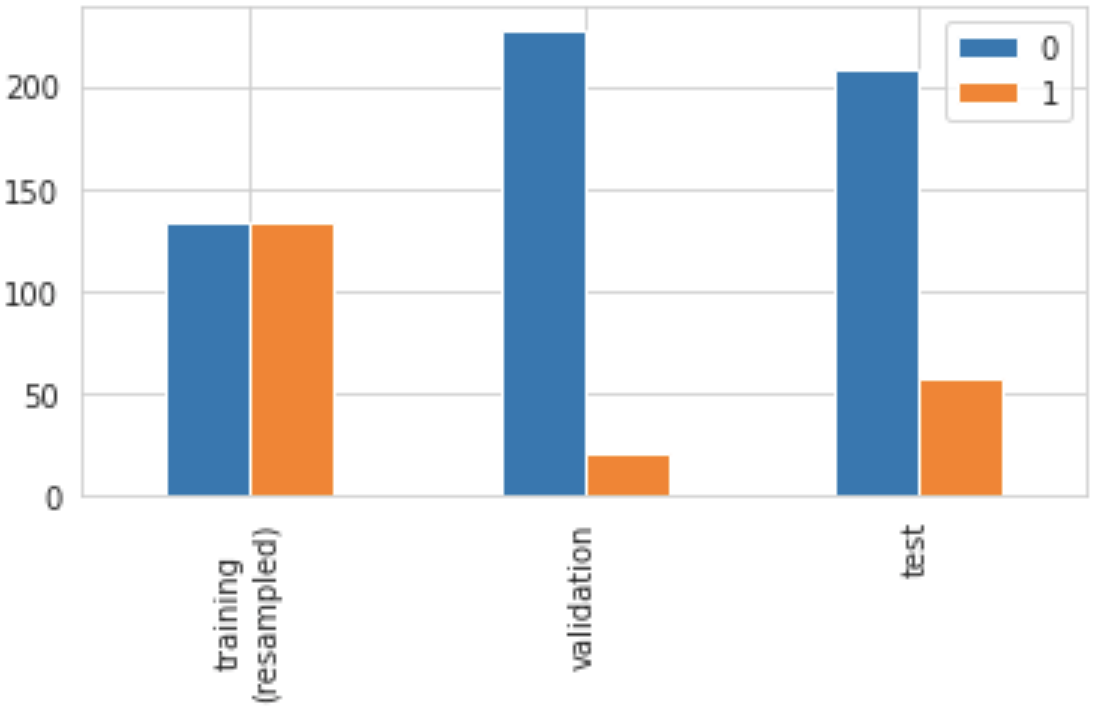
\includegraphics[height=5cm,keepaspectratio]{images/5_multimodal_fusion/proportion-splits.png}
\captionsetup{width=.95\textwidth}
\caption{Distribution of the dataset sizes. Training set has 134-134 both positive-negative samples. Validation set has 21-227 positive-negative samples. Test set has 57-208 positive-negative samples.}
\label{fig:proportion-splits}
\end{center}
\end{figure}



\subsection{Evaluation Metrics}

The classification task is a binary problem. This makes the evaluation metrics tied to the amount of correct and incorrect predictions. This is often summarized in a confusion matrix. See figure \ref{fig:confusion-matrix}. True positives and true negatives are predictions that are correctly classified. False positives are errors that are incorrectly marked as positive (i.e., the actual label is negative). Likewise, false negatives are errors that incorrectly marks as negative (i.e., the actual label is positive). From the amount of (in)correct predictions, we calculate the following metrics: Precision, Recall, F1 score and Average Precision.

\begin{figure}[ht]
\begin{center}
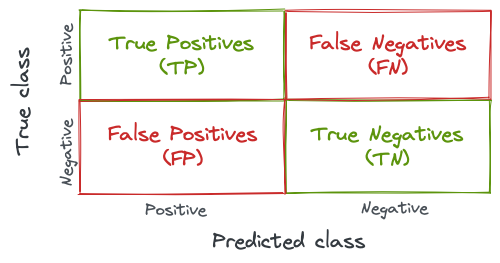
\includegraphics[width=0.5\textwidth,keepaspectratio]{images/5_multimodal_fusion/confusion-matrix.png}
\captionsetup{width=.95\textwidth}
\caption{Confusion matrix summarizes the performance of a classification task.}
\label{fig:confusion-matrix}
\end{center}
\end{figure}


\textbf{Precision} calculates the proportion of correct identified instances. It describes the correctness of positive classifications. Higher precision means that the model correctly classifies positive samples.

\begin{flalign*}
Precision = \frac{TP}{TP + FP} &&
\end{flalign*}

\textbf{Recall} calculates the proportion of positives that are identified. It describes the sensitivity of the model. Higher recall means that the model finds more positive samples.

\begin{flalign*}
Recall = \frac{TP}{TP + FN} &&
\end{flalign*}

\textbf{F1 score} combines precision and recall into one metric by calculating the harmonic mean between those metrics. It is possible to generalize F-score to give more importance to precision over recall, or vice-versa. In this thesis we use F1 score. 

\begin{flalign*}
F1 = \frac{2}{\frac{1}{Recall} \times \frac{1}{Precision}} &&
\end{flalign*}

\textbf{Average Precision} is the area under the precision recall curve (PRC). The precision recall curve visualizes the trade off between precision and recall at every possible recall threshold. See figure \ref{fig:precision-recall-curve} for illustration. Similar to the AP, often reported is the Area Under the Receiver Operator Curve (AUROC). However it is generally regarded that usage of AP is preferred over AUROC when the dataset is imbalanced \cite{Saito2015}.

\begin{figure}[ht]
\begin{center}
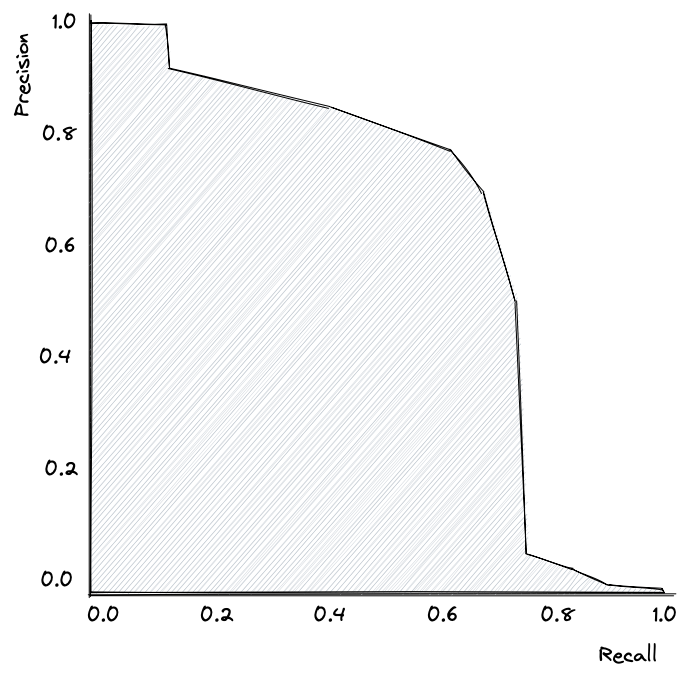
\includegraphics[height=4cm]{images/5_multimodal_fusion/precision-recall.png}
\end{center}
\captionsetup{width=0.95\textwidth}
\caption{Example of precision recall curve. The area under the curve is known a Average Precision.}
\label{fig:precision-recall-curve}
\end{figure}

\subsection{Track 1: Detecting Road Anomalies with Visual Data}
\label{sec:track-1-design}

The first track is to train a model solely using visual data to detect road anomalies. In this setting we can frame the task as object detection: classifying and locating defects in an image. As we know from literature survey (refer back to \ref{sec:object-detection}), YOLOv5 \cite{Jocher2021} is regarded as state-of-the-art for object detection. The authors provide various model configurations. Where each configuration differs in the size of the network.

During this track we train the visual model in two iterations. In the first iteration we train the original YOLO model to detect manholes. During this iteration the task is framed as object detection. We evaluate various configurations of YOLO. In the second iteration, we modify the best model to replace the object detection head. Instead, of detecting location of objects we want to compare the results with the other research tracks. Therefore, we replace the detection head with dense layers and frame it as binary classification task. 

The rest of the section is outlined as followed. We first explain how the data is prepared to train YOLO. Then, we discuss how an object detector evaluates predictions. Followed by description on the experiment setup, i.e., how YOLO is trained. Finally, we describe the second iteration. How the model is transformed from object detector to a binary classifier.

% \begin{figure}[ht]
% \begin{center}
% 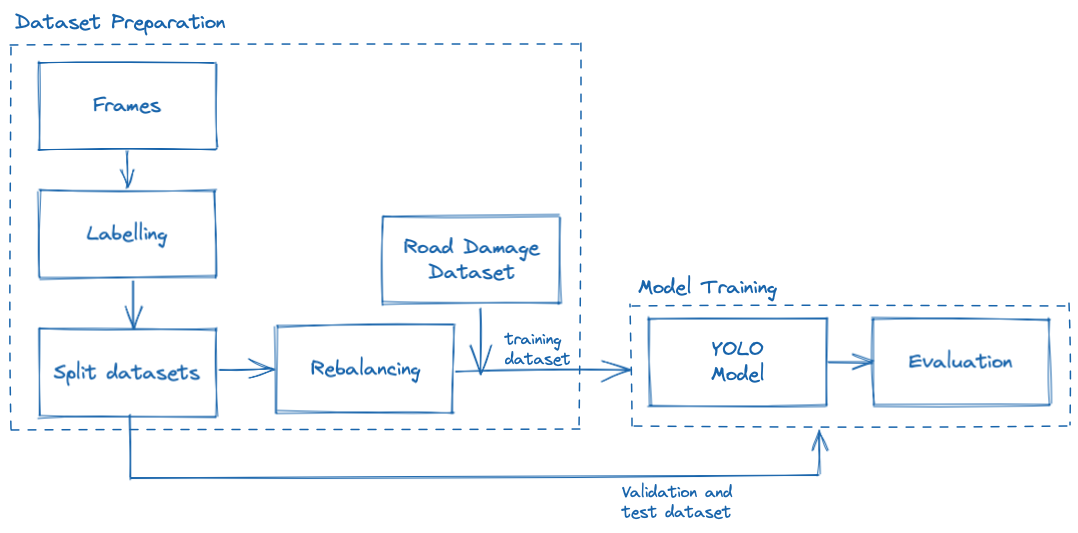
\includegraphics[width=0.95\textwidth,keepaspectratio]{images/5_multimodal_fusion/processing-overview-visual-model-2.png}
% \captionsetup{width=.95\textwidth}
% \caption{Overview of machine learning pipeline to detect visual damages.}
% \label{fig:visual-workflow}
% \end{center}
% \end{figure}


\subsubsection{Data Preparation}

As described earlier in section \ref{sec:visual-data}, visual data is annotated with CVAT \cite{cvat}. The labelled annotations are exported and converted from CVAT format to YOLO format. YOLO expects a certain dataset file (\code{dataset.yaml}) and directory structure to load the data. The dataset file describes which object classes exists, and allows configuration for hyperparameter tuning. Within the directory structure we have separate directories for training and validation data. Images containing one or multiple objects describe their respective objects in a label text file. In this label file, there is a single line for each object. The specification is \code{class x_center y_center width height}. Where \code{class} is the numeric index of the object class as defined in \code{dataset.yaml}. \code{x_center} and \code{y_center} describe the coordinates of the object, and \code{width} and \code{height} the size of the object. All values must be normalized between 0 and 1. Meaning that \code{x_center} and \code{width} are divided by the total width of the image, and \code{y_center} and \code{height} by the image height.

From literature we found a public dataset known as Road Damage Dataset \cite{Arya2020-competition}. This dataset contains annotated frames of road damages and manholes. The data was collected in Czechia, Japan, and India (see also section \ref{sec:visual-surface-defects}). During this track we supplement our training dataset with data from RDD. To this aim, we evaluate if we can improve our performance by introducing more data. The data from RDD is converted from Pascal VOC \cite{PascalVOC} format to YOLO format.


\subsubsection{Evaluating Classifications}

An object detector returns for an image all the detected objects. For each of the objects, the model returns: the detected class, the confidence, and the bounding box - that is where the object is located in the image. \textit{Intersection over Union} (IoU) is used to determine whether the model positively classified a detected object. IoU measures the overlap between the detected bounding box and the ground truth bounding box (i.e., the annotated area). IoU is calculated by the ratio of the \textit{area of intersection} over the total \textit{area of overlap}. This ratio is visually displayed in figure \ref{fig:iou}. When the IoU is above some threshold, the object is positively classified as that respective class. Common used value for threshold is 50\%.


\begin{figure}[ht]
\begin{center}
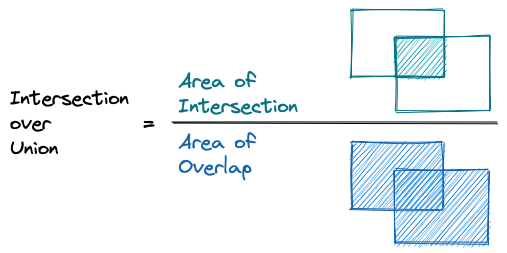
\includegraphics[height=4cm]{images/5_multimodal_fusion/IoU.png}
\end{center}
\captionsetup{width=0.95\textwidth}
\caption{Visualization describing the calculation of the Intersection over Union (IoU).}
\label{fig:iou}
\end{figure}


\subsubsection{Iteration 1: Training YOLO}

For the first iteration, we directly use the visual annotated frames as input, i.e., we skip the segmented dataset as described earlier. The frames are split into training (70\%), validation (21\%) and test split (9\%). The dataset is highly imbalanced: there are many more images without any anomalies. In object detection, images without an object are known as ``background images''.

From experience, object detection models are typically less sensitive to imbalanced datasets when there are multiple classes. However, an object detector does fail to learn when the majority of the images does not contain an object. Therefore in this iteration we resample the training dataset in majority of frames with objects. This is done by selecting at most x\% background images from each respective video. This yields an imbalanced dataset in favor of the object images. The author of YOLO also recommends to have small portion of background images to reduce false positives \cite{yolo-training-tips}. Note, we keep the original distribution for the validation and test set as it reflects the real world.

The author of YOLO provide various configuration of the model based on the network size. All configurations are pretrained on the COCO dataset \cite{COCO}. This is a object detection dataset, containing 80 classes. When training YOLO to detect different types of objects (e.g., manholes), it is recommended to transfer learn on pretrained models instead of training from scratch \cite{yolo-training-tips}. Unfortunately, training the model takes relatively long (multiple hours). It is therefore not trivial to perform cross validation or optimize for hyperparameters. Therefore we only experiment with YOLO on the following configurations: model size, image input size, proportion of background images, and proportion of RDD images.

Generally larger models perform better. The smallest model \code{YOLOv5s} has 1.9 million parameters, and the largest model \code{YOLOv5x} has 86.7 million parameters. YOLO internally resizes images to a configured input size. When larger image size is configured smaller objects are more visible. Both configurations affect the training time, and are limited to the available resources. Larger models and images require more GPU memory. Unfortunately our setup is relatively limited, thus we are not able to train all possible configurations. We select the largest possible batch size for each configuration without exceeding the available memory.

\subsubsection{Iteration 2: Modifying to Binary Classification}
\label{sec:modifying-yolo}

In order to compare the different tracks, we need to evaluate on the same dataset as described in section \ref{sec:dataset-setup}. To this aim, we modify the best performing YOLO model, and evaluate on the said segmented dataset. First, we export the trained model to Tensorflow \cite{yolo-export}. Then, we replace the object detection head of YOLO with dense layers: 128 nodes with ReLU activation, and 1 output node with sigmoid activation. See also figure \ref{fig:modified-yolo}. Finally, the modified model is trained on the segmented dataset. This modified model performs a binary classification task whether the input frame of the segment contains a manhole. 

Note, the layers of the YOLO model are frozen. This means that we keep the same parameters, and only train our replaced dense layers for binary classification. With this methodology we use the powerful YOLO model for feature extraction. The alternative approach is to train a network from scratch. However, transfer learning requires less resources e.g., less computational resources and less data \cite{Goodfellow2016}.


\begin{figure}[ht]
\begin{center}
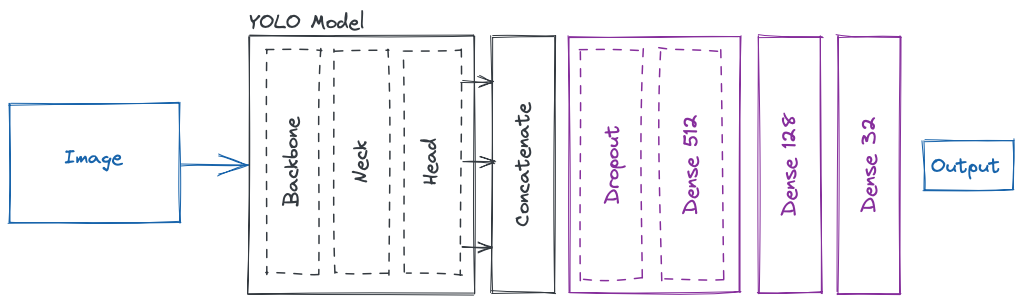
\includegraphics[width=.95\textwidth]{images/5_multimodal_fusion/modified-yolo-2.png}
\end{center}
\captionsetup{width=0.90\textwidth}
\caption{Architecture of the model for track 1: detecting manholes with visual data. It transfer learns retrained YOLO model to make binary classifications.}
\label{fig:modified-yolo}
\end{figure}



\subsection{Track 2: Detecting Road Anomalies with Accelerometer Data}
\label{sec:track-2-design}

In this track we aim to detect anomalies solely using accelerometer data. We train a model that accepts a short data sequence. The sequence is short segment extracted from the continuous accelerometer signal. The segment is classified as positive when the car drives over a manhole, otherwise it has a negative label. As described in section \ref{sec:dataset-setup}, segments are one second in length. As the accelerometer data is sampled at 100 Hz, this means each segment contains 100 samples.

The models are evaluated on two different inputs, either the raw input or after performing feature extraction. When training on raw data, we directly pass the data from a segment to the model. As the segments are 100 samples in length, this means that we have 300 inputs (three channels for each of the X, Y, and Z axis). 

The rest of this section describes the research design. We first explain the preprocessing operations such as feature extraction and feature scaling. Then, we describe the various machine learning models.


\subsubsection{Feature Extraction}

From earlier research we learned that Fast Fourier Transform (FFT) is often used as feature extractor for accelerometer data \cite{Hanson2014,Basavaraju2019,Wu2020,Janani2020}. Refer back to section \ref{sec:fft} for more information on FFT. In this track we also evaluate the effect of extracting features with FFT on model performance. For each segment, we perform the FFT on each of the respective accelerometer axes. 

We use scipy's \code{rfft} function to perform the calculation \cite{scipy}. When calculating Fourier transform on real signals, the output is mirrored in real and negative halves (in literature this is known as conjugate symmetry \cite{Smith1997}). Using \code{rfft} optimizes computation by only transforming the real half. The function returns complex numbers. In our case we are only interested in the presence of each frequency component. Thus, we calculate the magnitude of the complex number. This output is then used as input to the neural network. As we only use the real half, the input vector after feature extraction is 50 per channel (i.e., in total we have 150 inputs). See also listing \ref{list:feature_extraction} for more details.


\begin{minipage}{.95\textwidth}
\begin{lstlisting}[language=Python, caption={Pseudo implementation of performing feature extraction using FFT.}, label={list:feature_extraction}]
from scipy.fft import rfft

for ax in axes:
    # ax is the raw input (i.e., 100 samples)
    yt = rfft(ax)
    # yt is now of length 50 (only real half of signal)
    # abs calculates the magnitude of the complex vector
    yt = abs(yt)
\end{lstlisting}
\end{minipage}


\subsubsection{Feature Scaling} 

Using large values as input to a neural network leads to deteriorated performance. Models with large weights are usually unstable and are difficult to train \cite{Goodfellow2016}. Therefore we always perform feature scaling, regardless if we train the model on the raw acceleration data or after feature extraction. Feature scaling is done with function \code{StandardScaler} of scikit-learn's library \cite{scikit}. The function scales all features by subtracting the mean and dividing by the standard deviation.

\begin{flalign*}
Z_i = \frac{X_i - \mu}{\sigma} &&
\end{flalign*}


\subsubsection{Experiment Setup}

In this track we will train various deep neural networks to classify the segments. We also evaluate the performance of the networks based on the provided input. This either is the raw acceleration data or data after performing feature extraction (i.e., Fourier transform). There are endless possibilities when designing a neural network: how many hidden layers, how many nodes per layer, hyperparameters, etc. To scope our research we limit to three different types of architectures: Dense Neural Network (DNN), Convolutional Neural Network (CNN), and Long-Short Term Memory (LSTM). All models use Adam to optimize the gradients \cite{Kingma2014}. Learning rate is adjusted for each model for optimal performance. 

\begin{minipage}{\textwidth}
\textbf{Dense Neural Network}. Also referred to as fully connected network, is a basic multi-layer neural network. Each node in each layer is fully connected with each node in the following layer \cite{Goodfellow2016}. In this experiment we use a neural network with the following architecture. 1) the input layer is reshaped from 100 x 3 to wide shape of 300, 2) a block is constructed with a dense layer with $n$ nodes, dropout layer, and batch normalization layer. This block is repeated five times, where each following block has smaller node size, in this case: $256 \rightarrow 128 \rightarrow 64 \rightarrow 32$. The activation function of the dense layer is ReLU. 3) finally we have an output layer with sigmoid activation function. See also figure \ref{fig:dense-network}.
\vskip 1\baselineskip

\begin{center}
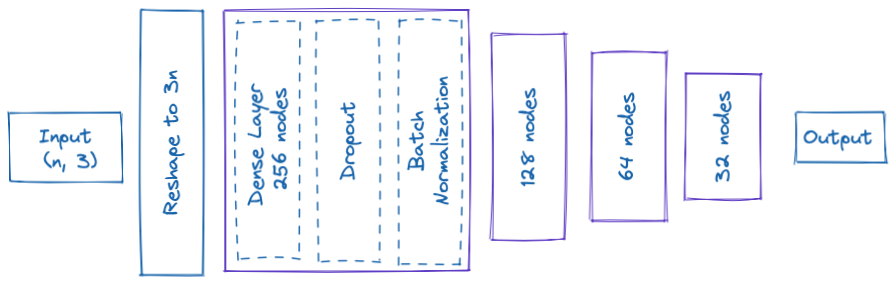
\includegraphics[height=5cm]{images/5_multimodal_fusion/dense-network-3.png}
\captionsetup{width=0.90\textwidth}
\captionof{figure}{Architecture of the Dense Neural Network. \textit{n} is 100 when raw input is passed, and 50 after applying feature extraction.}
\label{fig:dense-network}
\end{center}
\end{minipage}

\vskip 1\baselineskip

\begin{minipage}{\textwidth}
\textbf{Convolutional Neural Network}. With a CNN, the input is passed through one or multiple convolutional layers. A convolutional layer uses convolution kernels to convolve its inputs. It works as a filter and is then activated by non-linear activation function \cite{Goodfellow2016}. In this work we create the following network. 1) input of the three channels is directly passed through two convolutional layers. Both layers have 16 filters, a kernel size of 5, and ReLU as activation function, 2) the output of the filters is passed through Global Max Pooling layer, 3) subsequently two blocks of dense, dropout, and batch normalization are used (see above), 4) finally the output layer with the sigmoid activation function. See also figure \ref{fig:conv-network}. 
\vskip 1\baselineskip

\begin{center}
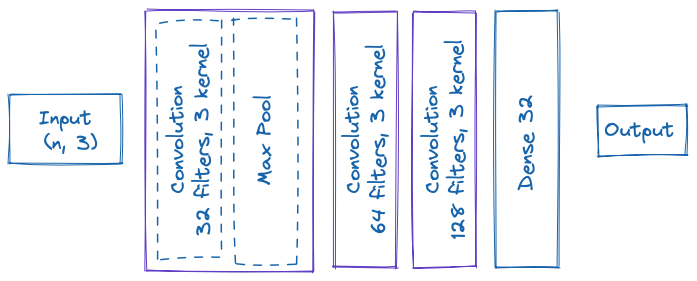
\includegraphics[height=5cm]{images/5_multimodal_fusion/convolution-network.png}
\captionsetup{width=0.90\textwidth}
\captionof{figure}{Architecture of the Convolutional Neural Network.}
\label{fig:conv-network}
\end{center}
\end{minipage}

\vskip 1\baselineskip

\begin{minipage}{\textwidth}
\textbf{Long-Short Term Memory}. A Recurrent Neural Network (RNN) can learn from the temporal relation between sensor readings. However RNN is very susceptible to gradient vanishing, making it difficult to learn. LSTM is variety of RNN. LSTM units allow gradients to flow unchanged. This makes LSTM networks able to learn long-term dependencies more easily \cite{Goodfellow2016}. LSTM networks are well suited for classifying time series data. We build our network as follows. 1) we have 3 LSTM layers with each 32 cells, 2) followed by dense layer of 32 nodes, 3) output. See also figure \ref{fig:lstm-network}.
\vskip 1\baselineskip

% \begin{figure}[ht]
\begin{center}
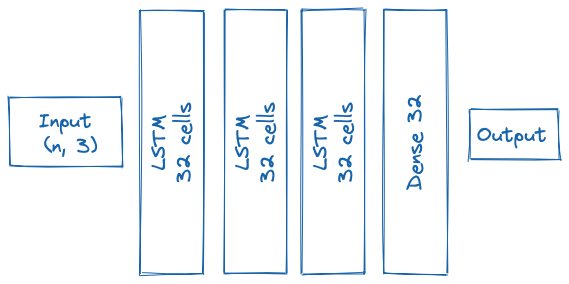
\includegraphics[height=5cm]{images/5_multimodal_fusion/lstm-network-2.png}
\captionsetup{width=0.90\textwidth}
\captionof{figure}{Architecture of the LSTM Network.}
\label{fig:lstm-network}
\end{center}
% \end{figure}
\end{minipage}


\subsection{Track 3: Detecting Road Anomalies with Multimodal Data}
\label{sec:track-3-design}

In the final track we combine the models of track 1 and track 2. In this track we train a model that takes both visual and accelerometer data from each segment as input, and predicts if the respective segment contains a manhole. During this track we evaluate both hybrid and late multimodal fusion. Refer back to section \ref{section:multimodal-ml} for more information about multimodal machine learning. Additionally, we design an experiment to validate that both data sources contribute to the outcome of the multimodal model.

\subsubsection{Experiment Setup}

First, we evaluate hybrid fusion (also called middle fusion). With hybrid fusion we aim to learn a joint representation inside the model. We concatenate the second last layers of both unimodal models. On this concatenated layer, we add a new detection head. This head consists of a dense layer with 32 nodes with ReLU activation. Followed by a single output node making the classification. The architecture of this network is shown in figure \ref{fig:multimodal-network}.

\begin{figure}[ht]
\begin{center}
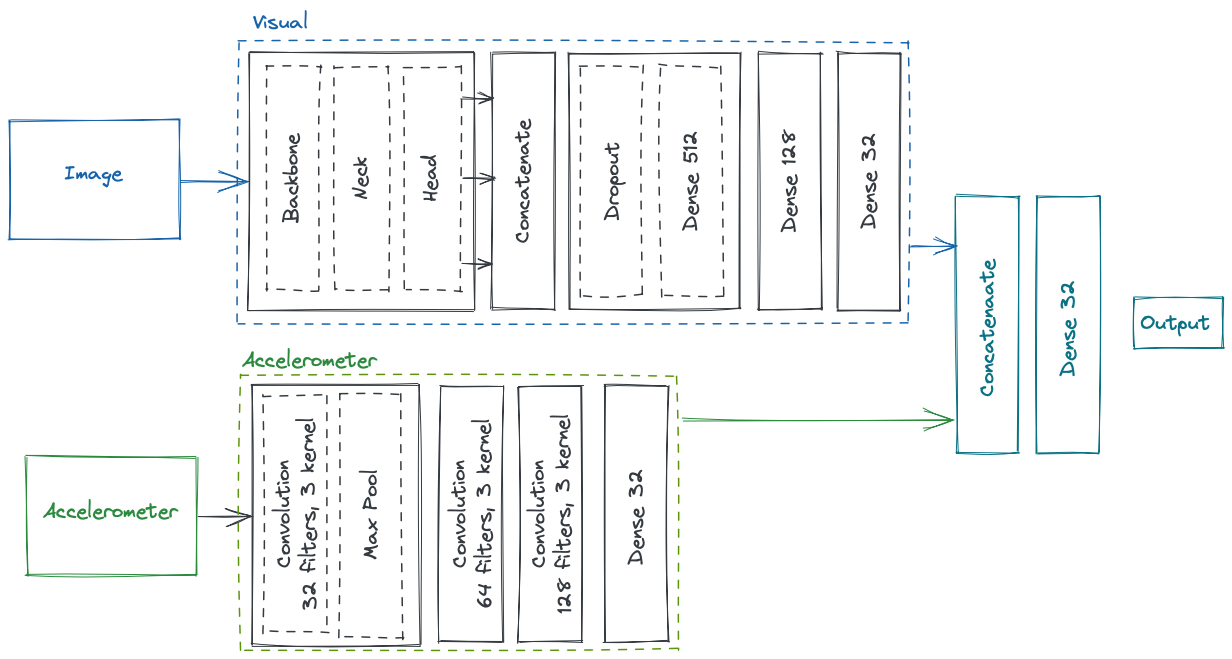
\includegraphics[width=0.95\textwidth]{images/5_multimodal_fusion/hybrid-fusion.png}
\captionsetup{width=0.90\textwidth}
\captionof{figure}{Architecture of the multimodal network.}
\label{fig:multimodal-network}
\end{center}
\end{figure}

Secondly, we evaluate late fusion. In this experiment we keep both unimodal models intact i.e., each model makes their respective classification. The outputs are combined with a voting classifier. In this case we average the prediction probabilities of both models. Predictions are positively labelled when the averaged probability exceeds the threshold of $0.5$. This method is also referred to as ensemble learning \cite{Baltrusaitis2017}.

Finally, we validate that the hybrid model learns from both data sources. We evaluate this by presenting the model with only one source of data. The other data source is zeroed out. For instance, we evaluate on the test with only providing visual data and z zeros for the accelerometer input. When the model learns a joint representation, we expect that the model still is able to make correct classifications \cite{Baltrusaitis2017}.

% \subsubsection{}

% \subsection{Capture Time Synchronization}
% \label{sec:capture-time-synchronization}


% \subsection{Distance Estimation}
% \label{sec:object-distance}


% \subsection{Moment Filtering}


% \subsection{Manhole Detection}
% Trained three models, at 100 epochs
% \begin{itemize}
% \item $YOLO_v5s$ at 1280 with batch 8
% \item $YOLO_v5m$ at 1280 with batch 4
% \item $YOLO_v5m$ at 640 with batch 16
% \end{itemize}

% The models with higher resolution (1280) perform relatively equal but much better than with the lower input size. Therefore we continue training only on larger inputs. 

% As the 1280 models are performing pretty similar, it makes sense to continue working with the s version. This YOLO model is smaller (less weights), but trains much quicker (86 min vs 226). 



% \subsection{ADR Cycle 1: Detecting Roadside Location Markers}

% With object detection the evaluation metrics measure how close the detected bounding boxes are to the ground-truth (labelled) bounding boxes. This measurement is done independently for each object class, by assessing the amount of overlap. Models are assessed on the following metrics: precision, recall and mAP \cite{Padilla2021}.

% Precision is ability to identify only relevant objects, the percentage of correct predictions. Recall is ability to find all relevant cases, the percentage of correct predictions among all given ground truths. In practice, we want a good object detector that find all ground truth objects (high recall), while only identifying relevant objects (high precision). Average Precision (MP) is metric based on the area below Precision x Recall curve. AP is obtained for each individual class, to yield a single metric, mean average precision (mAP) can be calculated by averaging the AP over all classes \cite{Padilla2021}.

% TODO: describe mAP calculation

% The first experiment is to detect roadside location markers, also known as \textit{hectometerpaal} or \textit{mile marker}. These are  small signs that are along the road to indicate the current position. See also figure \ref{fig:road-indicator} for an example of Dutch road location marker. The task is to detect the location and orientation of road indicators from the gathered data. With this output we can determine if the road location marker is in good condition, e.g. it is not skewed backwards but clearly visible.

% \begin{figure}[ht]
% \begin{center}
% 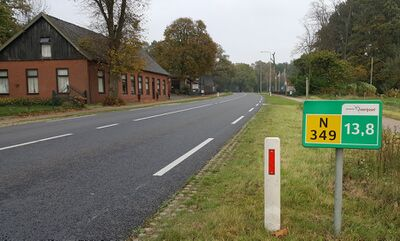
\includegraphics[height=4cm,keepaspectratio]{images/5_multimodal_fusion/example_hectometer.jpeg}
% \end{center}
% \caption{Example of roadside location marker (\textit{hectometerpaal}).}
% \end{figure}


% The reasons for this experiment are two-fold. First, the automation of detecting road sign damages. For road maintainers this is an easy optimization in their efficiency and thereby saves the road maintainers money. Second, although this is a relatively simple experiment, it enables the author to learn more about the practicalities of using YOLO, such as transfer learning, experiment tracking and resource utilization.


% \subsubsection{Setup}
% Classifying and locating objects is known as object detection. The output is the bounding box and class of the detected objects in an image. See also \ref{object-detection} for more information. Current state-of-the-art model for object detection is YOLOv5. This experiment uses YOLOv5 as model with pre-trained weights. The model is transfer learned to detect road side location markers. 

% At this time there were 536 annotated frames with visible roadside location markers. The data comes from three different trips, filmed with the same camera. The frames are split into a training, validation and test split. With respective proportions of 70\% / 21\% / 9\%. 


% \subsubsection{Results}
% The following configurations are tested:


% \begin{table}[h]
% \begin{tabular}{lllllll}
% Name                        & Model       & Image Size & Batch Size & Precision & Recall & mAP  \\
% last\_95\_img-640\_batch-42 & UCS-InfoLab & 640        & 4          & 0.74      & 0.55   & 0.62 \\
% yolo5m\_batch-640\_batch-4  & YOLOv5m     & 640        & 4          & 0.87      & 0.93   & 0.93 \\
% yolo5s\_batch-640\_batch-32 & YOLOv5s     & 640        & 32         & 0.59      & 0.61   & 0.56 \\
% yolo5s\_batch-640\_batch-16 & YOLOv5s     & 640        & 16         & 0.68      & 0.71   & 0.74 \\
% yolo5s\_batch-640\_batch-8  & YOLOv5s     & 640        & 8          & 0.80      & 0.78   & 0.86 \\
% yolo5s\_batch-1280\_batch-8 & YOLOv5s     & 1280       & 8           & \textbf{0.91} & \textbf{0.94} & \textbf{0.95}
% \end{tabular}
% \end{table}


% \begin{figure}[h]
% \begin{center}
% 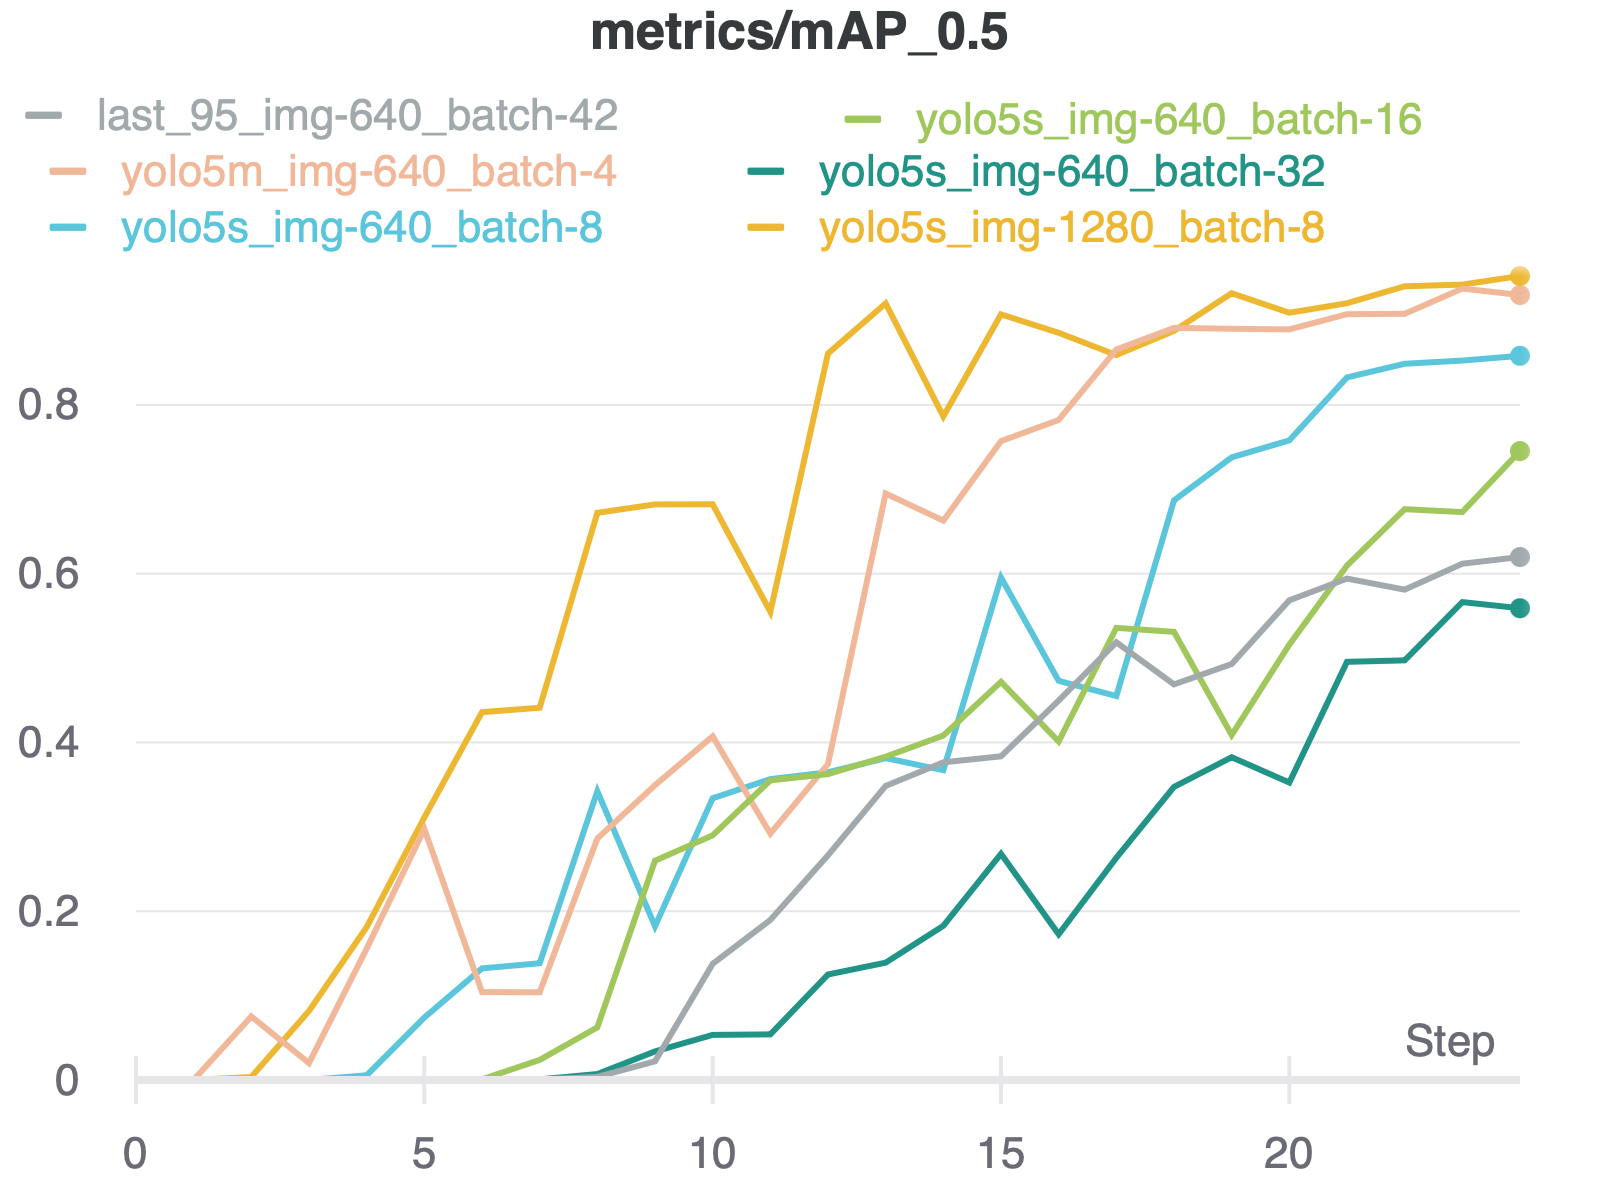
\includegraphics[height=4cm,keepaspectratio]{images/5_multimodal_fusion/exp-1_mAP.png}
% 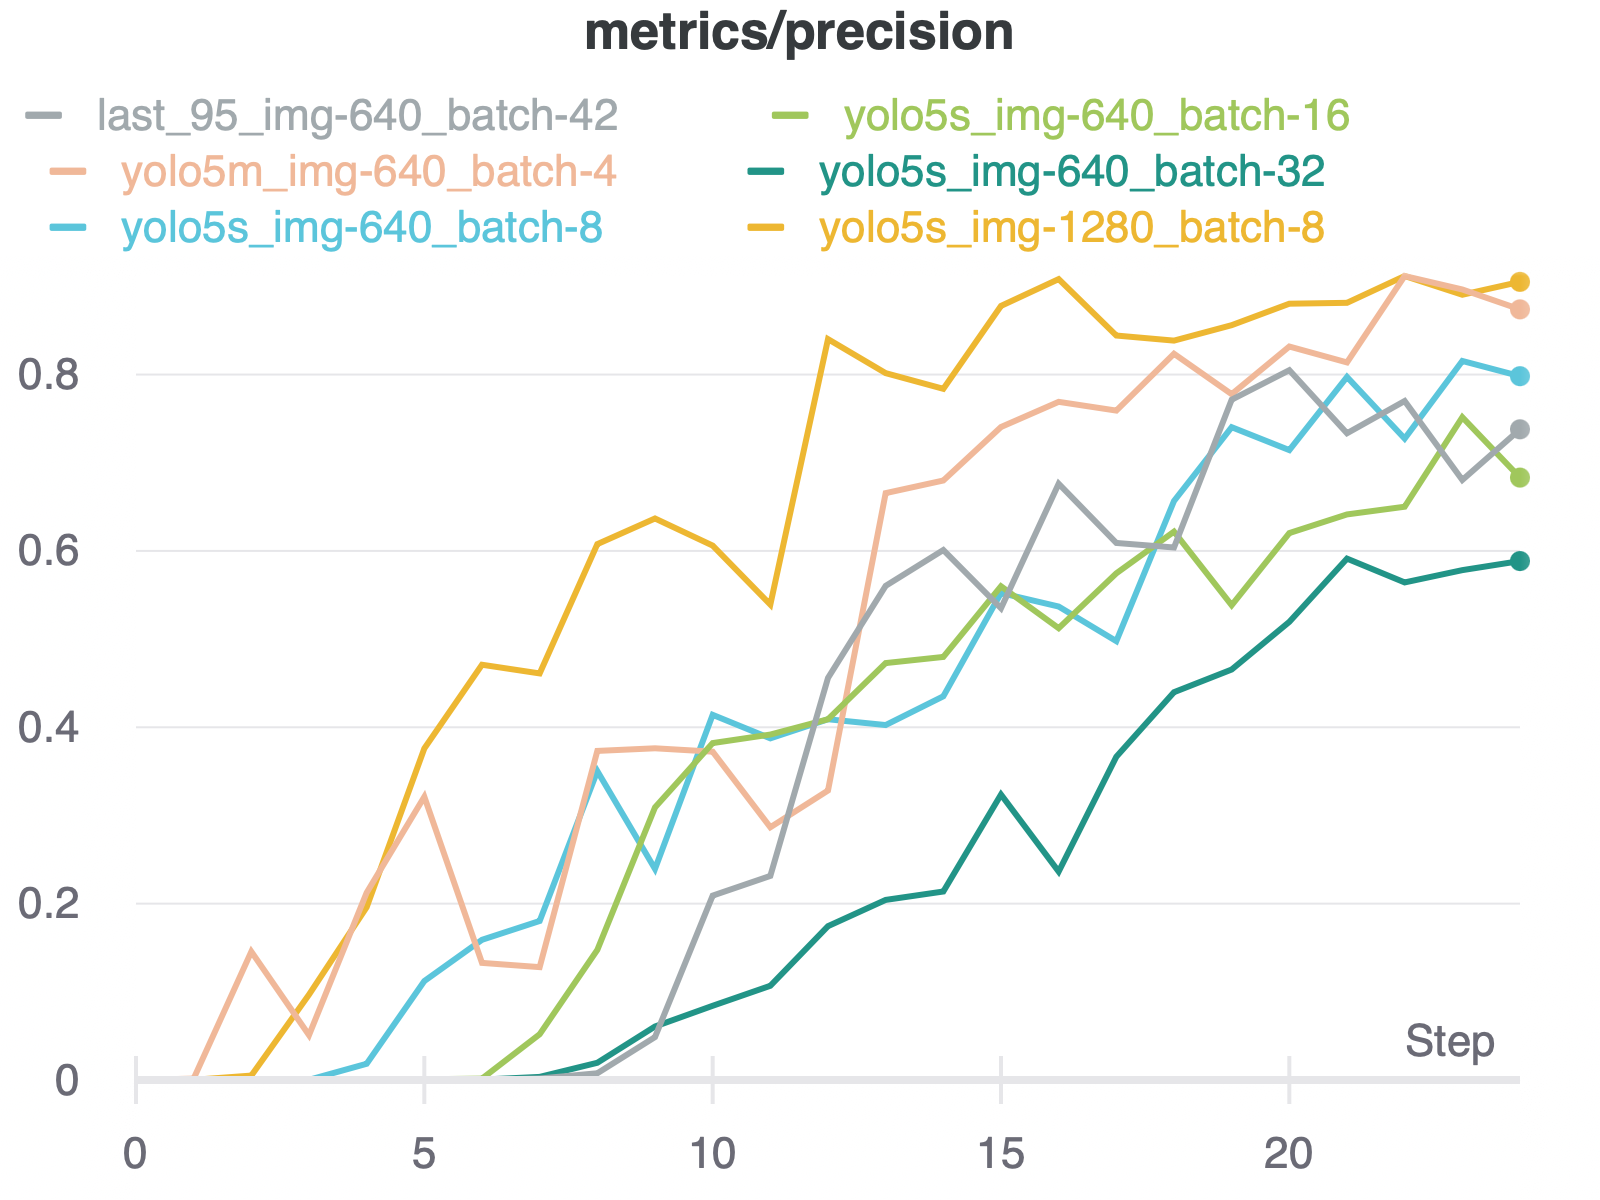
\includegraphics[height=4cm,keepaspectratio]{images/5_multimodal_fusion/exp-1_precision.png}
% 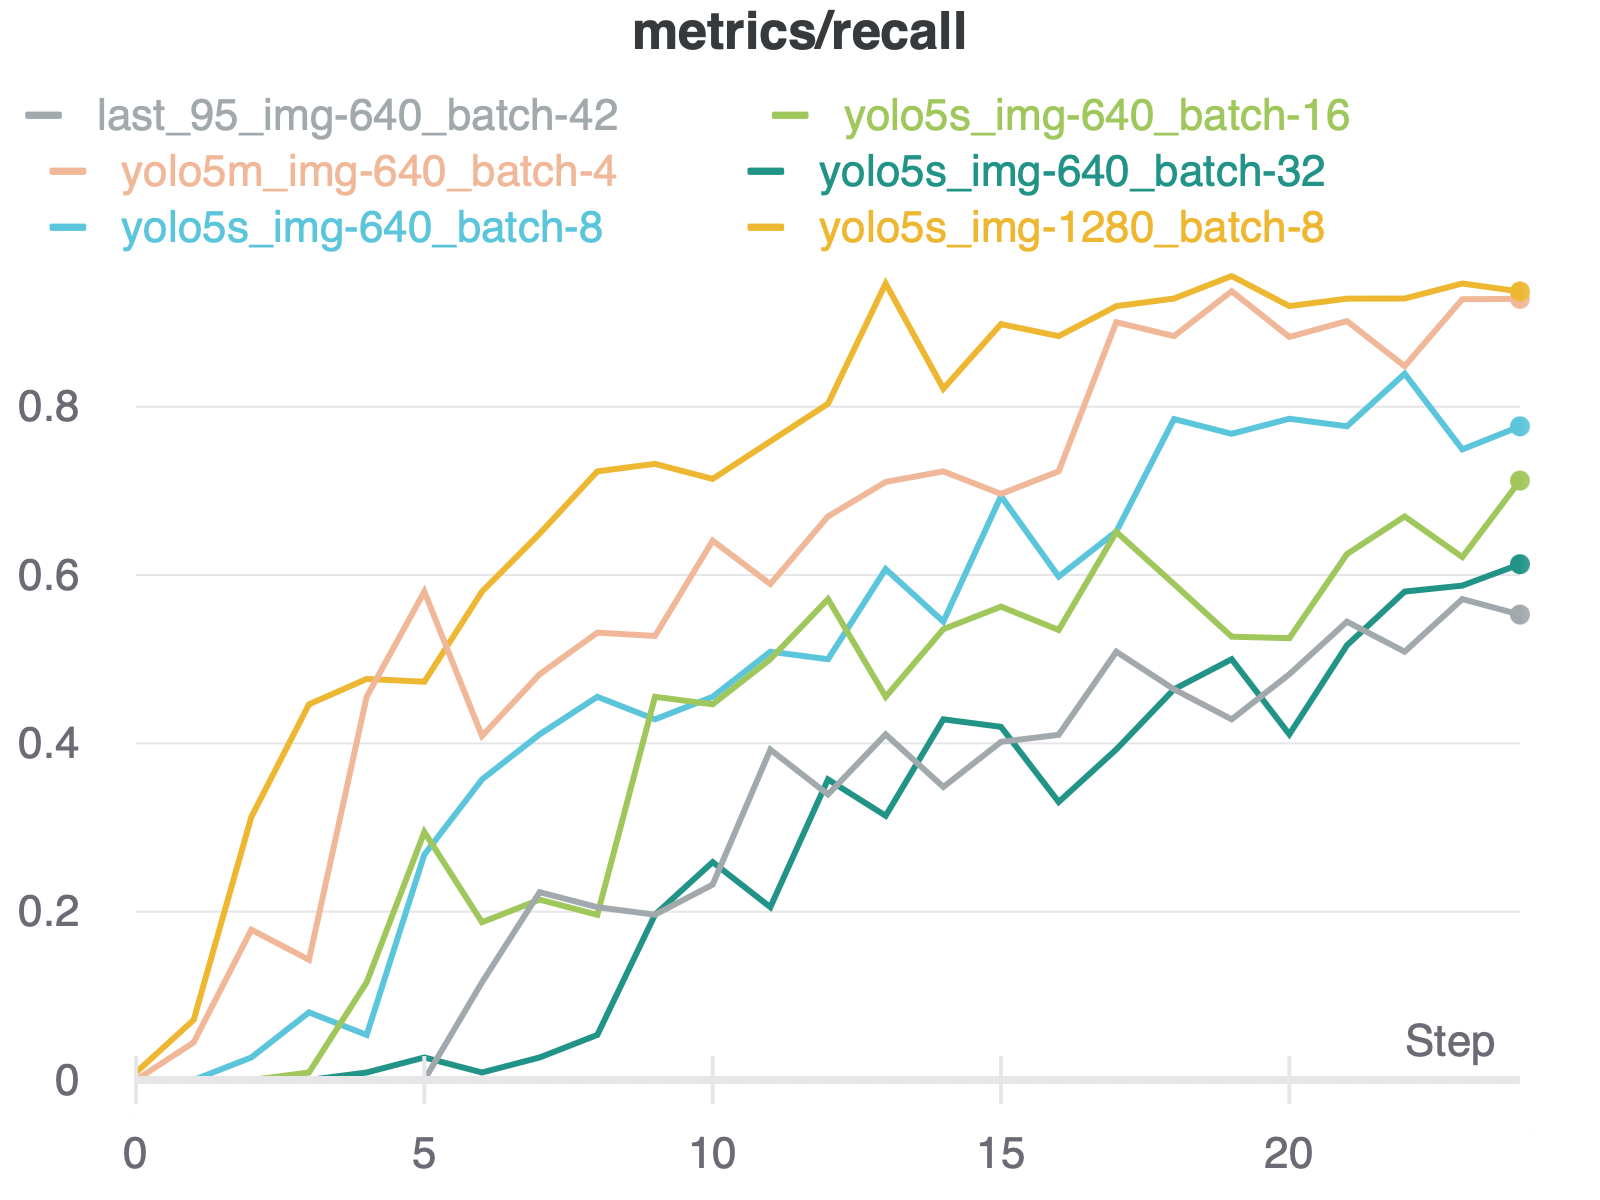
\includegraphics[height=4cm,keepaspectratio]{images/5_multimodal_fusion/exp-1_recall.png}
% \end{center}
% \caption{Experiment 1: performance metrics for detecting roadside location markers.}
% \end{figure}


% \textit{TODO: Describe the mislabelling and lower (omitted) mAP @ 0.5 scores}

% \begin{figure}[h]
% \begin{center}
% 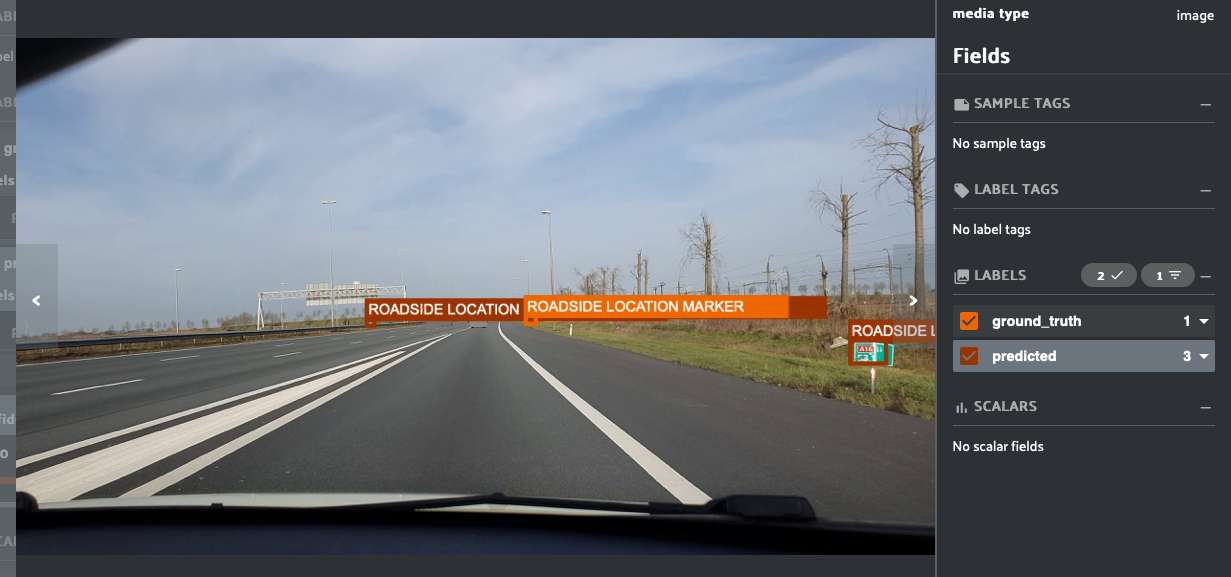
\includegraphics[width=\textwidth,keepaspectratio]{images/5_multimodal_fusion/exp-1_sample.png}
% \end{center}
% \caption{Example of predicted bounding boxes. Predicted boxes are in dark brown, while the ground truth labelling is in orange.}
% \end{figure}

% \subsubsection{Conclusion}

% Detecting roadside location markers appears to be a relatively easy task for YOLO. From the results table above we see that larger models perform better. In our task this seems explainable. The roadside location marker is relatively small in the whole image. Thus, a model with larger image size works best to detect these small objects.

% Although it is a simple experiment, during tests it appeared that the GPU might be a limiting factor for testing really large models. For completion, the aim was to test all possible configurations with YOLOv5s, YOLOv5m and image sizes in [640, 1280], and batch sizes in [4, 8, 16, 32]. Upon testing larger models (e.g. YOLOv5Mm with image size 1280), unfortunately the GPU experienced out of memory issues.


% \subsection{ADR Cycle 2: Estimate Vehicle-to-Object Distance }

% \subsection{ADR Cycle 3: Synchronize Visual and Accelerometer}

% \subsection{ADR Cycle 4: Train End-to-End Multimodal DL Model}
